%**************************************%
%* Generated from MathBook XML source *%
%*    on 2016-08-14T10:12:20-04:00    *%
%*                                    *%
%*   http://mathbook.pugetsound.edu   *%
%*                                    *%
%**************************************%
\documentclass[10pt,]{book}
%% Load geometry package to allow page margin adjustments
\usepackage{geometry}
\geometry{letterpaper,total={5.0in,9.0in}}
%% Custom Preamble Entries, early (use latex.preamble.early)
%% Inline math delimiters, \(, \), need to be robust
%% 2016-01-31:  latexrelease.sty  supersedes  fixltx2e.sty
%% If  latexrelease.sty  exists, bugfix is in kernel
%% If not, bugfix is in  fixltx2e.sty
%% See:  https://tug.org/TUGboat/tb36-3/tb114ltnews22.pdf
%% and read "Fewer fragile commands" in distribution's  latexchanges.pdf
\IfFileExists{latexrelease.sty}{}{\usepackage{fixltx2e}}
%% Page Layout Adjustments (latex.geometry)
%% This LaTeX file may be compiled with pdflatex, xelatex, or lualatex
%% The following provides engine-specific capabilities
%% Generally, xelatex and lualatex will do better languages other than US English
%% You can pick from the conditional if you will only ever use one engine
\usepackage{ifthen}
\usepackage{ifxetex,ifluatex}
\ifthenelse{\boolean{xetex} \or \boolean{luatex}}{%
%% begin: xelatex and lualatex-specific configuration
%% fontspec package will make Latin Modern (lmodern) the default font
\ifxetex\usepackage{xltxtra}\fi
\usepackage{fontspec}
%% realscripts is the only part of xltxtra relevant to lualatex 
\ifluatex\usepackage{realscripts}\fi
%% 
%% Extensive support for other languages
\usepackage{polyglossia}
\setdefaultlanguage{english}
%% Magyar (Hungarian)
\setotherlanguage{magyar}
%% Spanish
\setotherlanguage{spanish}
%% Vietnamese
\setotherlanguage{vietnamese}
%% end: xelatex and lualatex-specific configuration
}{%
%% begin: pdflatex-specific configuration
%% translate common Unicode to their LaTeX equivalents
%% Also, fontenc with T1 makes CM-Super the default font
%% (\input{ix-utf8enc.dfu} from the "inputenx" package is possible addition (broken?)
\usepackage[T1]{fontenc}
\usepackage[utf8]{inputenc}
%% end: pdflatex-specific configuration
}
%% Monospace font: Inconsolata (zi4)
%% Sponsored by TUG: http://levien.com/type/myfonts/inconsolata.html
%% See package documentation for excellent instructions
%% One caveat, seem to need full file name to locate OTF files
%% Loads the "upquote" package as needed, so we don't have to
%% Upright quotes might come from the  textcomp  package, which we also use
%% We employ the shapely \ell to match Google Font version
%% pdflatex: "varqu" option produces best upright quotes
%% xelatex,lualatex: add StylisticSet 1 for shapely \ell
%% xelatex,lualatex: add StylisticSet 2 for plain zero
%% xelatex,lualatex: we add StylisticSet 3 for upright quotes
%% 
\ifthenelse{\boolean{xetex} \or \boolean{luatex}}{%
%% begin: xelatex and lualatex-specific monospace font
\usepackage{zi4}
\setmonofont[BoldFont=Inconsolatazi4-Bold.otf,StylisticSet={1,3}]{Inconsolatazi4-Regular.otf}
%% end: xelatex and lualatex-specific monospace font
}{%
%% begin: pdflatex-specific monospace font
\usepackage[varqu]{zi4}
%% end: pdflatex-specific monospace font
}
%% Symbols, align environment, bracket-matrix
\usepackage{amsmath}
\usepackage{amssymb}
%% allow more columns to a matrix
%% can make this even bigger by overriding with  latex.preamble.late  processing option
\setcounter{MaxMatrixCols}{30}
%%
%% Color support, xcolor package
%% Always loaded.  Used for:
%% mdframed boxes, add/delete text, author tools
\PassOptionsToPackage{usenames,dvipsnames,svgnames,table}{xcolor}
\usepackage{xcolor}
%%
%% Semantic Macros
%% To preserve meaning in a LaTeX file
%% Only defined here if required in this document
%% Subdivision Numbering, Chapters, Sections, Subsections, etc
%% Subdivision numbers may be turned off at some level ("depth")
%% A section *always* has depth 1, contrary to us counting from the document root
%% The latex default is 3.  If a larger number is present here, then
%% removing this command may make some cross-references ambiguous
%% The precursor variable $numbering-maxlevel is checked for consistency in the common XSL file
\setcounter{secnumdepth}{3}
%% Environments with amsthm package
%% Theorem-like environments in "plain" style, with or without proof
\usepackage{amsthm}
\theoremstyle{plain}
%% Numbering for Theorems, Conjectures, Examples, Figures, etc
%% Controlled by  numbering.theorems.level  processing parameter
%% Always need a theorem environment to set base numbering scheme
%% even if document has no theorems (but has other environments)
\newtheorem{theorem}{Theorem}[section]
%% Only variants actually used in document appear here
%% Style is like a theorem, and for statements without proofs
%% Numbering: all theorem-like numbered consecutively
%% i.e. Corollary 4.3 follows Theorem 4.2
%% Definition-like environments, normal text
%% Numbering is in sync with theorems, etc
\theoremstyle{definition}
\newtheorem{definition}[theorem]{Definition}
%% Example-like environments, normal text
%% Numbering is in sync with theorems, etc
\theoremstyle{definition}
\newtheorem{example}[theorem]{Example}
%% Miscellaneous environments, normal text
%% Numbering for inline exercises and lists is in sync with theorems, etc
\theoremstyle{definition}
\newtheorem{exercise}[theorem]{Exercise}
%% Localize LaTeX supplied names (possibly none)
\renewcommand*{\proofname}{Proof}
\renewcommand*{\chaptername}{Chapter}
%% Figures, Tables, Listings, Floats
%% The [H]ere option of the float package fixes floats in-place,
%% in deference to web usage, where floats are totally irrelevant
%% We re/define the figure, table and listing environments, if used
%%   1) New mbxfigure and/or mbxtable environments are defined with float package
%%   2) Standard LaTeX environments redefined to use new environments
%%   3) Standard LaTeX environments redefined to step theorem counter
%%   4) Counter for new environments is set to the theorem counter before caption
%% You can remove all this figure/table setup, to restore standard LaTeX behavior
%% HOWEVER, numbering of figures/tables AND theorems/examples/remarks, etc
%% WILL ALL de-synchronize with the numbering in the HTML version
%% You can remove the [H] argument of the \newfloat command, to allow flotation and 
%% preserve numbering, BUT the numbering may then appear "out-of-order"
\usepackage{float}
\usepackage[bf]{caption} % http://tex.stackexchange.com/questions/95631/defining-a-new-type-of-floating-environment 
\usepackage{newfloat}
% Figure environment setup so that it no longer floats
\SetupFloatingEnvironment{figure}{fileext=lof,placement={H},within=section,name=Figure}
% figures have the same number as theorems: http://tex.stackexchange.com/questions/16195/how-to-make-equations-figures-and-theorems-use-the-same-numbering-scheme 
\makeatletter
\let\c@figure\c@theorem
\makeatother
%% Poetry Support
\newenvironment{poem}{\setlength{\parindent}{0em}}{}
\newcommand{\poemTitle}[1]{\begin{center}\large\textbf{#1}\end{center}}
\newcommand{\poemIndent}{\hspace{2 em}}
\newenvironment{stanza}{\vspace{0.25 em}\hangindent=4em}{\vspace{1 em}}
\newcommand{\stanzaTitle}[1]{{\centering\textbf{#1}\par}\vspace{-\parskip}}
\newcommand{\poemauthorleft}[1]{\vspace{-1em}\begin{flushleft}\textit{#1}\end{flushleft}}
\newcommand{\poemauthorcenter}[1]{\vspace{-1em}\begin{center}\textit{#1}\end{center}}
\newcommand{\poemauthorright}[1]{\vspace{-1em}\begin{flushright}\textit{#1}\end{flushright}}
\newcommand{\poemlineleft}[1]{{\raggedright{#1}\par}\vspace{-\parskip}}
\newcommand{\poemlinecenter}[1]{{\centering{#1}\par}\vspace{-\parskip}}
\newcommand{\poemlineright}[1]{{\raggedleft{#1}\par}\vspace{-\parskip}}
%% Raster graphics inclusion, wrapped figures in paragraphs
%% \resizebox sometimes used for images in side-by-side layout
\usepackage{graphicx}
%%
%% Program listing support, for inline code, Sage code
\usepackage{listings}
%% We define the listings font style to be the default "ttfamily"
%% To fix hyphens/dashes rendered in PDF as fancy minus signs by listing
%% http://tex.stackexchange.com/questions/33185/listings-package-changes-hyphens-to-minus-signs
\makeatletter
\lst@CCPutMacro\lst@ProcessOther {"2D}{\lst@ttfamily{-{}}{-{}}}
\@empty\z@\@empty
\makeatother
\ifthenelse{\boolean{xetex}}{}{%
%% begin: pdflatex-specific listings configuration
%% translate U+0080 - U+00F0 to their textmode LaTeX equivalents
%% Data originally from https://www.w3.org/Math/characters/unicode.xml, 2016-07-23
%% Lines marked in XSL with "$" were converted from mathmode to textmode
\lstset{extendedchars=true}
\lstset{literate={ }{{~}}{1}{¡}{{\textexclamdown }}{1}{¢}{{\textcent }}{1}{£}{{\textsterling }}{1}{¤}{{\textcurrency }}{1}{¥}{{\textyen }}{1}{¦}{{\textbrokenbar }}{1}{§}{{\textsection }}{1}{¨}{{\textasciidieresis }}{1}{©}{{\textcopyright }}{1}{ª}{{\textordfeminine }}{1}{«}{{\guillemotleft }}{1}{¬}{{\textlnot }}{1}{­}{{\-}}{1}{®}{{\textregistered }}{1}{¯}{{\textasciimacron }}{1}{°}{{\textdegree }}{1}{±}{{\textpm }}{1}{²}{{\texttwosuperior }}{1}{³}{{\textthreesuperior }}{1}{´}{{\textasciiacute }}{1}{µ}{{\textmu }}{1}{¶}{{\textparagraph }}{1}{·}{{\textperiodcentered }}{1}{¸}{{\c{}}}{1}{¹}{{\textonesuperior }}{1}{º}{{\textordmasculine }}{1}{»}{{\guillemotright }}{1}{¼}{{\textonequarter }}{1}{½}{{\textonehalf }}{1}{¾}{{\textthreequarters }}{1}{¿}{{\textquestiondown }}{1}{À}{{\`{A}}}{1}{Á}{{\'{A}}}{1}{Â}{{\^{A}}}{1}{Ã}{{\~{A}}}{1}{Ä}{{\"{A}}}{1}{Å}{{\AA }}{1}{Æ}{{\AE }}{1}{Ç}{{\c{C}}}{1}{È}{{\`{E}}}{1}{É}{{\'{E}}}{1}{Ê}{{\^{E}}}{1}{Ë}{{\"{E}}}{1}{Ì}{{\`{I}}}{1}{Í}{{\'{I}}}{1}{Î}{{\^{I}}}{1}{Ï}{{\"{I}}}{1}{Ð}{{\DH }}{1}{Ñ}{{\~{N}}}{1}{Ò}{{\`{O}}}{1}{Ó}{{\'{O}}}{1}{Ô}{{\^{O}}}{1}{Õ}{{\~{O}}}{1}{Ö}{{\"{O}}}{1}{×}{{\texttimes }}{1}{Ø}{{\O }}{1}{Ù}{{\`{U}}}{1}{Ú}{{\'{U}}}{1}{Û}{{\^{U}}}{1}{Ü}{{\"{U}}}{1}{Ý}{{\'{Y}}}{1}{Þ}{{\TH }}{1}{ß}{{\ss }}{1}{à}{{\`{a}}}{1}{á}{{\'{a}}}{1}{â}{{\^{a}}}{1}{ã}{{\~{a}}}{1}{ä}{{\"{a}}}{1}{å}{{\aa }}{1}{æ}{{\ae }}{1}{ç}{{\c{c}}}{1}{è}{{\`{e}}}{1}{é}{{\'{e}}}{1}{ê}{{\^{e}}}{1}{ë}{{\"{e}}}{1}{ì}{{\`{\i}}}{1}{í}{{\'{\i}}}{1}{î}{{\^{\i}}}{1}{ï}{{\"{\i}}}{1}{ð}{{\dh }}{1}{ñ}{{\~{n}}}{1}{ò}{{\`{o}}}{1}{ó}{{\'{o}}}{1}{ô}{{\^{o}}}{1}{õ}{{\~{o}}}{1}{ö}{{\"{o}}}{1}{÷}{{\textdiv }}{1}{ø}{{\o }}{1}{ù}{{\`{u}}}{1}{ú}{{\'{u}}}{1}{û}{{\^{u}}}{1}{ü}{{\"{u}}}{1}{ý}{{\'{y}}}{1}{þ}{{\th }}{1}{ÿ}{{\"{y}}}{1}}
%% end: pdflatex-specific listings configuration
}
%% End of generic listing adjustments
%% Sage's blue is 50%, we go way lighter (blue!05 would work)
\definecolor{sageblue}{rgb}{0.95,0.95,1}
%% Sage input, listings package: Python syntax, boxed, colored, line breaking
%% Indent from left margin, flush at right margin
\lstdefinestyle{sageinput}{language=Python,breaklines=true,breakatwhitespace=true,basicstyle=\small\ttfamily,columns=fixed,frame=single,backgroundcolor=\color{sageblue},xleftmargin=4ex}
%% Sage output, similar, but not boxed, not colored
\lstdefinestyle{sageoutput}{language=Python,breaklines=true,breakatwhitespace=true,basicstyle=\small\ttfamily,columns=fixed,xleftmargin=4ex}
%% Multiple column, column-major lists
\usepackage{multicol}
%% More flexible list management, esp. for references and exercises
%% But also for specifying labels (i.e. custom order) on nested lists
\usepackage{enumitem}
%% Lists of references in their own section, maximum depth 1
\newlist{referencelist}{description}{4}
\setlist[referencelist]{leftmargin=!,labelwidth=!,labelsep=0ex,itemsep=1.0ex,topsep=1.0ex,partopsep=0pt,parsep=0pt}
%% Lists of exercises in their own section, maximum depth 4
\newlist{exerciselist}{description}{4}
\setlist[exerciselist]{leftmargin=0pt,itemsep=1.0ex,topsep=1.0ex,partopsep=0pt,parsep=0pt}
%% Indented groups of exercises within an exercise section, maximum depth 4
\newlist{exercisegroup}{description}{4}
\setlist[exercisegroup]{leftmargin=2em,labelindent=2em,itemsep=1.0ex,topsep=1.0ex,partopsep=0pt,parsep=0pt}
%% Support for index creation
%% imakeidx package does not require extra pass (as with makeidx)
%% We set the title of the "Index" section via a keyword
%% And we provide language support for the "see" phrase
\usepackage{imakeidx}
\makeindex[title=Index, intoc=true]
\renewcommand{\seename}{see}
%% Package for tables spanning several pages
\usepackage{longtable}
%% hyperref driver does not need to be specified
\usepackage{hyperref}
%% configure hyperref's  \url  to match listings' inline verbatim
\renewcommand\UrlFont{\small\ttfamily}
%% Hyperlinking active in PDFs, all links solid and blue
\hypersetup{colorlinks=true,linkcolor=blue,citecolor=blue,filecolor=blue,urlcolor=blue}
\hypersetup{pdftitle={Applied Discrete Structures}}
%% If you manually remove hyperref, leave in this next command
\providecommand\phantomsection{}
%% If tikz has been loaded, replace ampersand with \amp macro
%% extpfeil package for certain extensible arrows,
%% as also provided by MathJax extension of the same name
%% NB: this package loads mtools, which loads calc, which redefines
%%     \setlength, so it can be removed if it seems to be in the 
%%     way and your math does not use:
%%     
%%     \xtwoheadrightarrow, \xtwoheadleftarrow, \xmapsto, \xlongequal, \xtofrom
%%     
%%     we have had to be extra careful with variable thickness
%%     lines in tables, and so also load this package late
\usepackage{extpfeil}
%% Custom Preamble Entries, late (use latex.preamble.late)
%% Begin: Author-provided macros
%% (From  docinfo/macros  element)
%% Plus three from MBX for XML characters
\newcommand{\identity}{\mathrm{id}}
\newcommand{\notdivide}{{\not{\mid}}}
\newcommand{\notsubset}{\not\subset}
\newcommand{\lcm}{\operatorname{lcm}}
\newcommand{\gf}{\operatorname{GF}}
\newcommand{\inn}{\operatorname{Inn}}
\newcommand{\aut}{\operatorname{Aut}}
\newcommand{\Hom}{\operatorname{Hom}}
\newcommand{\cis}{\operatorname{cis}}
\newcommand{\chr}{\operatorname{char}}
\newcommand{\Null}{\operatorname{Null}}
\newcommand{\lt}{ < }
\newcommand{\gt}{ > }
\newcommand{\amp}{ & }
%% End: Author-provided macros
%% Title page information for book
\title{Applied Discrete Structures}
\author{Al Doerr\\
Department of Mathematical Sciences\\
University of Massachusetts Lowell\\
\href{mailto:}{\nolinkurl{}}
\and
Ken Levasseur\\
Department of Mathematical Sciences\\
University of Massachusetts Lowell\\
\href{mailto:kenneth_levasseur@uml.edu}{\nolinkurl{kenneth_levasseur@uml.edu}}
}
\date{September, 2016}
\begin{document}
\frontmatter
%% begin: half-title
\thispagestyle{empty}
{\centering
\vspace*{0.28\textheight}
{\Huge Applied Discrete Structures}\\}
\clearpage
%% end:   half-title
%% begin: adcard
\thispagestyle{empty}
\null%
\clearpage
%% end:   adcard
%% begin: title page
%% Inspired by Peter Wilson's "titleDB" in "titlepages" CTAN package
\thispagestyle{empty}
{\centering
\vspace*{0.14\textheight}
{\Huge Applied Discrete Structures}\\[3\baselineskip]
{\Large Al Doerr}\\[0.5\baselineskip]
{\Large University of Massachusetts Lowell}\\[3\baselineskip]
{\Large Ken Levasseur}\\[0.5\baselineskip]
{\Large University of Massachusetts Lowell}\\[3\baselineskip]
{\Large September, 2016}\\}
\clearpage
%% end:   title page
%% begin: copyright-page
\thispagestyle{empty}
\vspace*{\stretch{2}}
\noindent\textcopyright\ 2016\quad{}Al Doerr, Ken Levasseur\\[0.5\baselineskip]
Applied Discrete Structures by Alan Doerr and Kenneth Levasseur is licensed under a Creative Commons Attribution-NonCommercial-ShareAlike 3.0 United States License. You are free to Share: copy and redistribute the material in any medium or format; Adapt: remix, transform, and build upon the material. You may not use the material for commercial purposes.  The licensor cannot revoke these freedoms as long as you follow the license terms.
			\par
\vspace*{\stretch{1}}
\null\clearpage
%% end:   copyright-page
%% begin: acknowledgement
\chapter*{Acknowledgements}\label{acknowledgement-1}
\addcontentsline{toc}{chapter}{Acknowledgements}
I would like to thank Rob Beezer, David Farmer and other participants on the \href{https://groups.google.com/forum/?fromgroups#!forum/mathbook-xml-support}{mathbook-xml-support group} for their guidance and work on MathBook XML.  Thanks to the Pedagogy Subcommittee of the UMass Lowell Transformational Education Committee for their financial assistance in helping getting this project started.%
%% end:   acknowledgement
%% begin: preface
\chapter*{Preface}\label{preface-1}
\addcontentsline{toc}{chapter}{Preface}
This version of \emph{Applied Discrete Structures} is being developed using \emph{Mathbook XML}, A lightweight XML application for authors of scientific articles, textbooks and monographs initiated by Rob Beezer, U. of Puget Sound.  %
\par
Sage (\href{http://sagemath.org}{sagemath.org}) is a free, open source, software system for advanced mathematics.  Sage can be used either on your own computer, a local server, or on SageMathCloud (\href{https://cloud.sagemath.com}{https://cloud.sagemath.com}). %
\par\hfill\begin{tabular}{l@{}}
Ken Levasseur\\
Lowell MA
\end{tabular}\\\par
%% end:   preface
%% begin: table of contents
\setcounter{tocdepth}{1}
\renewcommand*\contentsname{Contents}
\tableofcontents
%% end:   table of contents
\mainmatter
\typeout{************************************************}
\typeout{Chapter 1 Combinatorics}
\typeout{************************************************}
\chapter[Combinatorics]{Combinatorics}\label{combinatorics}
\typeout{************************************************}
\typeout{Introduction  }
\typeout{************************************************}
\begin{poem}
\poemTitle{Enumerative Combinatorics}
\begin{stanza}
\poemlineleft{Enumerative combinatorics}
\poemlineleft{Date back to the first prehistorics}
\poemlineleft{Who counted; relations}
\poemlineleft{Like sets' permutations}
\poemlineleft{To them were part cult, part folklorics.}
\end{stanza}
\poemauthorleft{Michael ToalsterThe Omnificent English Dictionary In Limerick Form}
\end{poem}
Throughout this book we will be counting things. In this chapter we will outline some of the tools that will help us count.%
\par
Counting occurs not only in highly sophisticated applications of mathematics to engineering and computer science but also in many basic applications. Like many other powerful and useful tools in mathematics, the concepts are simple; we only have to recognize when and how they can be applied.
%
\typeout{************************************************}
\typeout{Section 1.1 Basic Counting Techniques - The Rule of Products}
\typeout{************************************************}
\section[Basic Counting Techniques - The Rule of Products]{Basic Counting Techniques - The Rule of Products}\label{the-rule-of-products}
\typeout{************************************************}
\typeout{Subsection 1.1.1 What is Combinatorics?}
\typeout{************************************************}
\subsection[What is Combinatorics?]{What is Combinatorics?}\label{What-is-Combinatorics}

 One of the first concepts our parents taught us was the ``art of counting.'' We were taught to raise three fingers to indicate that we were three years old. The question of ``how many'' is a natural and frequently asked question. Combinatorics is the ``art of counting.'' It is the study of techniques that will help us to count the number of objects in a set quickly. Highly sophisticated results can be obtained with this simple concept. The following examples will illustrate that many questions concerned with counting involve the same process.
%
\begin{example}[How many lunches can you have?]\label{lunch-possibilies1}
A snack bar serves five different sandwiches and three different beverages. How many different lunches can a person order? One way of determining the number of possible lunches is by listing or enumerating all the possibilities. One systematic way of doing this is by means of a tree, as in the following figure.%
\leavevmode%
\begin{figure}
\centering
\includegraphics[width=1\linewidth]{images/lunch.png}
\caption{Tree diagram to enumerate the number of possible lunches.
                \label{lunch}}
\end{figure}
\par

 Every path that begins at the position labeled START and goes to the right can be interpreted as a choice of one of the five sandwiches followed by a choice of one of the three beverages. Note that considerable work is required to arrive at the number fifteen this way; but we also get more than just a number. The result is a complete list of all possible lunches. If we need to answer a question that starts with ``How many . . . ,'' enumeration would be done only as a last resort. In a later chapter we will examine more enumeration techniques.
%
\par

 An alternative method of solution for this example is to make the simple observation that there are five different choices for sandwiches and three different choices for beverages, so there are \(5 \cdot 3 = 15\) different lunches that can be ordered.
%
\par

 A listing of possible lunches a person could have is: \({(BEEF, milk), (BEEF, juice), (BEEF, coffee), ..., (BOLOGNA, coffee)}\).
%
\end{example}
\begin{example}[Counting elements in a cartesion product]\label{cartesian-cardinality}
Let \(A = \{a, b, c, d, e\}\) and \(B = \{1,2,3\}\). From Chapter 1 we know how to list the elements in \(A \times B = \{(a, 1), (a, 2), (a, 3), ..., (e, 3)\}\).  Since the first entry of each pair can be any one of the five elements \(a, b, c, d\), and \(e\), and since the second can be any one of the three numbers 1, 2, and 3, it is quite clear there are 
\(5 \cdot 3 = 15\) different elements in \(A \times B\).
%
\end{example}
\begin{example}[A True-False Questionnaire]\label{questionnaire}
A person is to complete a true-false questionnaire consisting of ten questions. How many different ways are there to answer the questionnaire? Since each question can be answered either of two ways (true or false), and there are a total of ten questions, there are \begin{equation*} 2 \cdot 2 \cdot 2 \cdot 2 \cdot 2 \cdot 2 \cdot 2 \cdot 2 \cdot 2 \cdot 2 = 2^{10} = 1024\end{equation*} different ways of answering the questionnaire. The reader is encouraged to visualize the tree diagram of this example, but not to draw it!%
\end{example}
\par

 We formalize the procedures developed in the previous examples with the following rule and its extension.
%
\typeout{************************************************}
\typeout{Subsection 1.1.2 The Rule Of Products:}
\typeout{************************************************}
\subsection[The Rule Of Products:]{The Rule Of Products:}\label{rule-of-products}
\index{The Rule Of Products:}If two operations must be performed, and If the first operation can always be performed \(p_1\) different ways and the second operation can always be performed \(p_2\) different ways, then there are \(p_1 p_2\) different ways that the two operations can be performed.
%
\par

Note: It is important that \(p_2\) does not depend on the option that is chosen in the first operation. Another way of saying this is that \(p_2\) is independent of the first operation. If \(p_2\) is dependent on the first operation, then the rule of products does not apply.
%
\begin{example}[Reduced Lunch Possibilities]\label{lunch-possibilites2}
Assume in \hyperref[lunch-possibilies1]{\ref{lunch-possibilies1}}, coffee is not served with a beef or chicken sandwiches. Then by inspection of \hyperref[lunch]{\ref{lunch}} we see that there are only thirteen different choices for lunch. The rule of products does not apply, since the choice of beverage depends on one's choice of a sandwich.%
\end{example}
\par
\emph{Extended Rule Of Products.} The rule of products can be extended to include sequences of more than two operations. If \(n\) operations must be performed, and the number of options for each operation is \(p_1\), \(p_2, \dots, p_n\) respectively, with each \(p_i\)  independent of previous choices, then the \(n\) operations can be performed \(p_1 \cdot p_2 \cdot \cdots \cdot p_n\) different ways.
%
\begin{example}[A Multiple Choice Questionnaire]\label{another_questionnaire}
A questionnaire contains four questions that have two possible answers and three questions with five possible answers. Since the answer to each question is independent of the answers to the other questions, the extended rule of products applies and there are
\(2 \cdot 2 \cdot 2 \cdot 2 \cdot 5 \cdot 5 \cdot 5 = 2^4 \cdot 5^3 = 2000 \) different ways to answer the questionnaire.%
\end{example}
\par

 In Chapter 1 we introduced the power set of a set A, P(A), which is the set of all subsets of A. Can we predict how many elements are in \(\mathcal{P}(A)\) for a given finite set A? The answer is yes, and in fact if \(\lvert A \rvert  = n\), then \(\mathcal{P}(A) = 2^{n}\).  The ease with which we can prove this fact demonstrates the power and usefulness of the rule of products. Do not underestimate the usefulness of simple ideas.
%
\begin{theorem}[Power Set Cardinality Theorem]\label{power-set-cardinality-theorem}
\index{Power Set Cardinality Theorem}If \(A\) is a finite set, then \(\lvert \mathcal{P}(A) \rvert = 2^{\lvert A \rvert }\).%
\end{theorem}
\begin{proof}\hypertarget{proof-1}{}

Proof: Consider how we might determine any \(B \in \mathcal{P}(A)\), where \( \lvert A \rvert =n\). For each element \(x \in A\) there are two choices, either \(x \in B\) or \(x \notin B\).  Since there are \(n\)  elements of \(A\)  we have, by the rule of products, 
  \begin{equation*}\underset{n \textrm{ factors}}{\underline{2 \cdot 2 \cdot  \cdots \cdot 2}}=  2^n\end{equation*}   different subsets of \(A\). Therefore, \(\mathcal{P}(A)= 2^{n}\).
%
\end{proof}
\typeout{************************************************}
\typeout{Exercises 1.1.3 Exercises}
\typeout{************************************************}
\subsection[Exercises]{Exercises}\label{EXERCISES-FOR-SECTION-2-1}
\hypertarget{exercisegroup-1}{}\typeout{************************************************}
\typeout{Introduction  }
\typeout{************************************************}
A Exercises%
\begin{exercisegroup}
\item[1.]\hypertarget{exercise-1}{} In horse racing, to bet the ``daily double'' is to select the winners of the first two races of the day. You win only if both selections are correct. In terms of the number of horses that are entered in the first two races, how many different daily double bets could be made?%
\par\smallskip
\par\smallskip
\noindent\textbf{Answer.}\hypertarget{answer-1}{}\quad
 If there are \(m\) horses in race 1 and \(n\) horses in race 2 then there are \(m \cdot n\) possible daily doubles.%
\item[2.]\hypertarget{exercise-2}{} Professor Shortcut records his grades using only his students' first and last initials. What is the smallest class size that will definitely force Prof. S. to use a different system?%
\par\smallskip
\item[3.]\hypertarget{exercise-3}{}  A certain shirt comes in four sizes and six colors. One also has the choice of a dragon, an alligator, or no emblem on the pocket. How many different shirts could you order?%
\par\smallskip
\par\smallskip
\noindent\textbf{Answer.}\hypertarget{answer-2}{}\quad
  \(72=4\cdot 6\cdot 3\)%
\item[4.]\hypertarget{exercise-4}{}  A builder of modular homes would like to impress his potential customers with the variety of styles of his houses. For each house there are blueprints for three different living rooms, four different bedroom configurations, and two different garage styles. In addition, the outside can be finished in cedar shingles or brick. How many different houses can be designed from these plans?%
\par\smallskip
\item[5.]\hypertarget{exercise-5}{}  The Pi Mu Epsilon mathematics honorary society of Outstanding University wishes to have a picture taken of its six officers. There will be two rows of three people. How many different way can the six officers be arranged?%
\par\smallskip
\par\smallskip
\noindent\textbf{Answer.}\hypertarget{answer-3}{}\quad
 \(720=6\cdot 5\cdot 4\cdot 3\cdot 2\cdot 1\)%
\item[6.]\hypertarget{exercise-6}{} An automobile dealer has several options available for each of three different packages of a particular model car: a choice of two styles of seats in three different colors, a choice of four different radios, and five different exteriors. How many choices of automobile does a customer have?%
\par\smallskip
\item[7.]\hypertarget{exercise-7}{} A clothing manufacturer has put out a mix-and-match collection consisting of two blouses, two pairs of pants, a skirt, and a blazer. How many outfits can you make? Did you consider that the blazer is optional? How many outfits can you make if the manufacturer adds a sweater to the collection?%
\par\smallskip
\par\smallskip
\noindent\textbf{Answer.}\hypertarget{answer-4}{}\quad
If we always include the blazer in the outfit we would have 6 outfits. If we
consider the blazer optional then there would be 12 outfits. When we add a
sweater we have the same type of choice. Considering the sweater optional
produces 24 outfits.%
\item[8.]\hypertarget{exercise-8}{} As a freshman, suppose you had to take two of four lab science courses, one of two literature courses, two of three math courses, and one of seven physical education courses. Disregarding possible time conflicts, how many different schedules do you have to choose from?%
\par\smallskip
\item[9.]\hypertarget{exercise-9}{} (a) Suppose each single character stored in a computer uses eight bits. Then each character is represented by a different sequence of eight 0's and l's called a bit pattern. How many different bit patterns are there? (That is, how many different characters could be represented?)%
\par
 (b) How many bit patterns are palindromes (the same backwards as forwards)?%
\par
 (c) How many different bit patterns have an even number of 1's?%
\par\smallskip
\par\smallskip
\noindent\textbf{Answer.}\hypertarget{answer-5}{}\quad
\leavevmode%
\begin{enumerate}[label=\alph*]
\item\hypertarget{li-1}{} \(2^8=256\)%
\item\hypertarget{li-2}{} \(2^4=16\). Here we are concerned only with the first four bits, since the last four must be the same.%
\item\hypertarget{li-3}{} \(2^7=128\), you have no choice in the last bit.%
\end{enumerate}
%
\item[10.]\hypertarget{exercise-10}{} Automobile license plates in Massachusetts usually consist of three digits followed by three letters. The first digit is never zero. How many different plates of this type could be made?%
\par\smallskip
\item[11.]\hypertarget{exercise-11}{} (a) Let \(A = \{1, 2, 3, 4\}\). Determine the number of different subsets of \(A\).%
\par
 (b) Let \(A = \{1, 2, 3, 4, 5\}\). Determine the number of proper subsets of \(A\) .%
\par\smallskip
\par\smallskip
\noindent\textbf{Answer.}\hypertarget{answer-6}{}\quad
\leavevmode%
\begin{multicols}{2}
\begin{enumerate}[label=\alph*]
\item\hypertarget{li-4}{}\(16\)%
\item\hypertarget{li-5}{} \(30\)%
\end{enumerate}
\end{multicols}
%
\item[12.]\hypertarget{exercise-12}{} How many integers from 100 to 999 can be written with no 7's?%
\par\smallskip
\item[13.]\hypertarget{exercise-13}{} Consider three persons, A, B, and C, who are to be seated in a row of three chairs. Suppose A and B are identical twins. How many seating arrangements of these persons can there be%
\par
\leavevmode%
\begin{multicols}{2}
\begin{enumerate}[label=\alph*]
\item\hypertarget{li-6}{} If you are a total stranger?%
\item\hypertarget{li-7}{} If you are A and B's mother?%
\end{enumerate}
\end{multicols}
%
\par
This problem is designed to show you that different people can have different correct answers to the same problem.%
\par\smallskip
\par\smallskip
\noindent\textbf{Answer.}\hypertarget{answer-7}{}\quad
\leavevmode%
\begin{multicols}{2}
\begin{enumerate}[label=\alph*]
\item\hypertarget{li-8}{}\(3\)%
\item\hypertarget{li-9}{}\(\ 6\)%
\end{enumerate}
\end{multicols}
%
\item[14.]\hypertarget{exercise-14}{}How many ways can a student do a ten-question true-false exam if he or she can choose not to answer any number of questions?%
\par\smallskip
\item[15.]\hypertarget{exercise-15}{} Suppose you have a choice of fish, lamb, or beef for a main course, a choice of peas or carrots for a vegetable, and a choice of pie, cake, or ice cream for dessert. If you must order one item from each category, how many different dinners are possible?%
\par\smallskip
\par\smallskip
\noindent\textbf{Answer.}\hypertarget{answer-8}{}\quad
\(18\)%
\item[16.]\hypertarget{exercise-16}{} Suppose you have a choice of vanilla, chocolate, or strawberry for ice cream, a choice of peanuts or walnuts for chopped nuts, and a choice of hot fudge or marshmallow for topping. If you must order one item from each category, how many different sundaes are possible?%
\par\smallskip
\end{exercisegroup}
\par\smallskip\noindent
\hypertarget{exercisegroup-2}{}\typeout{************************************************}
\typeout{Introduction  }
\typeout{************************************************}
B Exercises%
\begin{exercisegroup}
\item[17.]\hypertarget{exercise-17}{} A questionnaire contains six questions each having yes-no answers. For each yes response, there is a follow-up question with four possible responses.%
\par
\leavevmode%
\begin{enumerate}[label=\alph*]
\item\hypertarget{li-10}{}Draw a tree diagram that illustrates how many ways a single question in the questionnaire can be answered.%
\item\hypertarget{li-11}{}How many ways can the questionnaire be answered?%
\end{enumerate}
%
\par\smallskip
\par\smallskip
\noindent\textbf{Answer.}\hypertarget{answer-9}{}\quad
\leavevmode%
\begin{figure}
\centering
\includegraphics[width=1\linewidth]{images/fig-sol-2-1-17.png}
\end{figure}

\leavevmode%
\begin{enumerate}[label=\alph*]
\item\hypertarget{li-12}{}See \hyperref[fig-sol-2-1-17]{Figure~}%
\item\hypertarget{li-13}{}\(5^6\)%
\end{enumerate}
%
\item[18.]\hypertarget{exercise-18}{} Ten people are invited to a dinner party. How many ways are there of seating them at a round table? If the ten people consist of five men and five women, how many ways are there of seating them if each man must be surrounded by two women around the table?%
\par\smallskip
\item[19.]\hypertarget{exercise-19}{} How many ways can you separate a set with \(n\)  elements into two nonempty subsets if the order of the subsets is immaterial? What if the order of the subsets is important?%
\par\smallskip
\par\smallskip
\noindent\textbf{Answer.}\hypertarget{answer-10}{}\quad
\(2^{n-1}-1\) and \(2^n-2\)%
\item[20.]\hypertarget{exercise-20}{} A gardener has three flowering shrubs and four nonflowering shrubs. He must plant these shrubs in a row using an alternating pattern, that is, a shrub must be of a different type from that on either side. How many ways can he plant these shrubs? If he has to plant these shrubs in a circle using the same pattern, how many ways can he plant this circle? Note that one nonflowering shrub will be left out at the end.%
\par\smallskip
\end{exercisegroup}
\par\smallskip\noindent
\typeout{************************************************}
\typeout{Section 1.2 Permutations}
\typeout{************************************************}
\section[Permutations]{Permutations}\label{permutations}

 A number of applications of the rule of products are of a specific type, and because of their frequent appearance they are given their own designation, permutations. Consider the following examples.
%
\begin{example}[Ordering the elements of a set]\label{ordering_a_set}
How many different ways can we order the three different elements of the set \(A = \{a, b, c\}\)? Since we have three choices for position one, two choices for position two, and one choice for the third position, we have, by the rule of products, \(3 \cdot 2 \cdot 1 = 6\) different ways of ordering the three letters. We illustrate through a tree diagram.%
\leavevmode%
\begin{figure}
\centering
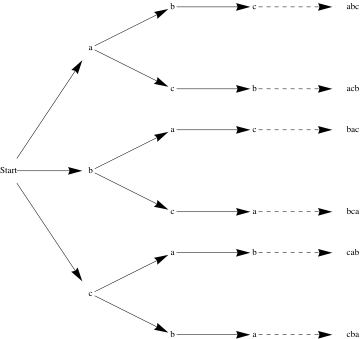
\includegraphics[width=1\linewidth]{images/tree-of-permutations.png}
\caption{A tree to enumerate permutations of a three element set.
                \label{tree-of-permutations}}
\end{figure}
\par

 Each of the six orderings is called a permutation of the set A.
%
\end{example}
\begin{example}[Ordering a schedule]\label{ordering_a_schedule}
A student is taking five courses in the fall semester. How many different ways can the five courses be listed? There are \(5 \cdot 4 \cdot 3 \cdot 2 \cdot 1 = 120\) different permutations of the set of courses.%
\end{example}
\par
In each of the above examples of the rule of products we observe that:%
\par
\leavevmode%
\begin{enumerate}
\item\hypertarget{li-14}{}We are asked to order or arrange elements from a single set.%
\item\hypertarget{li-15}{}Each element is listed exactly once in each list (permutation). So if there are \(n\) choices for position one in a list, there are \(n - 1\) choices for position two, \(n - 2\) choices for position three, etc.%
\end{enumerate}
%
\begin{example}[Some orderings of a baseball team]\label{some_orderings_of_a_baseball_team}
The alphabetical ordering of the players of a baseball team is one permutation of the set of players. Other orderings of the players' names might be done by batting average, age, or height. The information that determines the ordering is called the key. We would expect that each key would give a different permutation of the names. If there are twenty-five players on the team, there are \(25 \cdot 24 \cdot 23 \cdot \cdots  \cdot 3 \cdot 2 \cdot 1\) different permutations of the players.%
\par
This number of permutations is huge. In fact it is 15511210043330985984000000, but writing it like this isn't all that instructive, while leaving it as a product as we originally had makes it easier to see where the number comes from.  We just need to find a more compact way of writing these products.%
\end{example}
\par

 We now develop notation that will be useful for permutation problems.
%
\begin{definition}[Factorial]\label{Definition-Factorial.}
\index{Factorial}\label{notation-1}
If \(n\) is a positive integer then \(n\) factorial is the product of the first \(n\) positive integers and is denoted \(n!\). Additionally, we define zero factorial, \(0!\) to be 1.%
\end{definition}
\par
The first few factorials are 
\begin{equation*}
\begin{array}{ccccccccc}
 n & 0 & 1 & 2 & 3 & 4 & 5 & 6 &
   7 \\
  n! & 1 & 1 & 2 & 6 & 24 & 120 &
   720 & 5040 \\
\end{array}
\end{equation*}%
\par
Note that \(4!\) is 4 times \(3!\), or 24, and \(5!\) is 5 times \(4!\), or 120. In addition, note that as n grows in size, \(n!\) grows extremely quickly. For example, \(11! = 39916800\). If the answer to a problem happens to be \(25!\), as in the previous example, you would never be expected to write that number out completely. However, a problem with an answer of \(\frac{25!}{23!}\) can be reduced to \(25 \cdot 24\), or 600.%
\par

 If \(\lvert A \rvert = n \), there are \(n!\) ways of permuting all \(n\)  elements of \(A\) . We next consider the more general situation where we would like to permute \(k\) elements  out of a set of \(n\)  objects, where \( k \leq n\).
%
\begin{example}[Choosing Club Officers]\label{choosing-club-officers}
A club of twenty-five members will hold an election for president, secretary, and treasurer in that order. Assume a person can hold only one position. How many ways are there of choosing these three officers? By the rule of products there are \(25 \cdot 24 \cdot 23\) ways of making a selection.%
\end{example}
\begin{definition}[Permutation]\label{permutation}
\index{Permutation} An ordered arrangement of \(k\) elements selected from a set of \(n\) elements, \(0 \leq k \leq  n\), where no two elements of the arrangement are the same, is called a permutation of \(n\) objects taken \(k\) at a time. The total number of such permutations is denoted by \(P(n, k)\).%
\end{definition}
\begin{theorem}[Permutation Counting Formula]\label{permutations-counting-formula}
\index{Permutation Counting Formula} The number of possible permutations of \(k\)  elements taken from a set of \(n\)  elements is
 \begin{equation*}P(n,k)=n \cdot (n-1) \cdot (n-2) \cdot  \cdots  \cdot (n-k+1) = \prod_{j=0}^{k-1} (n-j) = \frac{n!}{(n-k)!} \end{equation*}%
\end{theorem}
\begin{proof}\hypertarget{proof-2}{}
  Case I: If \(k = m\) we have \(P(n,n)=n!=\frac{n!}{(n-n)!}\). %
\par
 Case II: If \(0 \leq  k < n\),then we have \(k\)  positions to fill using \(n\) elements and%
\par
\leavevmode%
\begin{enumerate}
\item\hypertarget{li-16}{}
 Position 1 can be filled by any one of \(n-0=n\)  elements
%
\item\hypertarget{li-17}{}
 Position 2 can be filled by any one of \(n-1\)  elements
%
\item\hypertarget{li-18}{}\( \cdots \)%
\item\hypertarget{li-19}{}
 Position k can be filled by any one of \(n-(k-1)=n-k+1\)  elements
%
\end{enumerate}
%
\par
Hence, by the rule of products, \begin{equation*}P(n,k) = n \cdot(n - 1) \cdot (n - 2) \cdot \cdots \cdot (n - k + 1) = \frac{n!}{(n-k)!}\end{equation*}. %
\end{proof}
\par

 It is important to note that the derivation of the permutation formula given above was done solely through the rule of products. This serves to reiterate our introductory remarks in this section that permutation problems are really rule-of-products problems.  We close this section with several examples.
%
\begin{example}[Another example of choosing officers]\label{more_club_officers}
A club has eight members eligible to serve as president, vice-president, and treasurer. How many ways are there of choosing these officers?
%
\par

 Solution 1: Using the rule of products. There are eight possible choices for the presidency, seven for the vice-presidency, and six for the office of treasurer. By the rule of products there are \(8 \cdot 7\cdot 6 = 336\) ways of choosing these officers.
%
\par

 Solution 2: Using the permutation formula. We want the total number of permutations of eight objects taken three at a time:
 	\begin{equation*}P(8,3)=\frac{8!}{(8-3)!}=8 \cdot 7 \cdot 6 = 336\end{equation*}
%
\end{example}
\begin{example}[Course ordering, revisited]\label{course-ordering-revisited}
To count the number of ways to order five courses, we can use the permutation formula. We want the number of permutations of five courses taken five at a time:
\begin{equation*}P(5,5)= \frac{5!}{(5-5)!}= 5!= 120\end{equation*}%
\end{example}
\begin{example}[Ordering of digits under different conditions]\label{ordering-digits}
Consider only the digits 1, 2, 3, 4, and 5.%
\par
\leavevmode%
\begin{enumerate}[label=\alph*]
\item\hypertarget{li-20}{} How many three-digit numbers can be formed if no repetition of digits can occur?%
\item\hypertarget{li-21}{} How many three-digit numbers can be formed if repetition of digits is allowed?%
\item\hypertarget{li-22}{} How many three-digit numbers can be formed if only non-consecutive repetition of digits are allowed?%
\end{enumerate}
%
\par

 Solutions to (a): Solution 1: Using the rule of products. We have any one of five choices for digit one, any one of four choices for digit two, and three choices for digit three. Hence, \(5 \cdot 4 \cdot 3 = 60\) different three-digit numbers can be formed.
%
\par
Solution 2; Using the permutation formula. We want the total number of permutations of five digits taken three at a time:
 \begin{equation*}P(5,3)=\frac{5!}{(5-3)!}=5 \cdot 4 \cdot 3 = 60\end{equation*}%
\par
Solution to (b): The definition of permutation indicates `` ...no two elements in each list are the same.'' Hence the permutation formula cannot be used. However, the rule of products still applies. We have any one of five choices for the first digit, five choices for the second, and five for the third. So there are \(5 \cdot 5\cdot 5 = 125\) possible different three-digit numbers if repetition is allowed.%
\par
Solution to (c): Again, the rule of products applies here. We have any one of five choices for the first digit, but then for the next two digits we have four choices since we are not allowed to repeat the previous digit  So there are \(5 \cdot 4\cdot 4 = 80\) possible different three-digit numbers if only non-consecutive repetitions are allowed.%
\end{example}
\typeout{************************************************}
\typeout{Exercises 1.2.1 Exercises}
\typeout{************************************************}
\subsection[Exercises]{Exercises}\label{exercises-2}
\hypertarget{exercisegroup-3}{}\typeout{************************************************}
\typeout{Introduction  }
\typeout{************************************************}
A Exercises%
\begin{exercisegroup}
\item[1.]\hypertarget{exercise-21}{} If a raffle has three different prizes and there are 1,000 raffle tickets sold, how many different ways can the prizes be distributed?%
\par\smallskip
\par\smallskip
\noindent\textbf{Answer.}\hypertarget{answer-11}{}\quad
 \(P(1000,3)\)%
\item[2.]\hypertarget{exercise-22}{}\leavevmode%
\begin{enumerate}[label=\alph*]
\item\hypertarget{li-23}{} How many three-digit numbers can be formed from the digits 1, 2, 3 if no repetition of digits is allowed? List the three-digit numbers.%
\item\hypertarget{li-24}{}How many two-digit numbers can be formed if no repetition of digits is allowed? List them.%
\item\hypertarget{li-25}{}How many two-digit numbers can be obtained if repetition is allowed?%
\end{enumerate}
%
\par\smallskip
\item[3.]\hypertarget{exercise-23}{} How many eight-letter words can be formed from the 26 letters in the alphabet? Even without concerning ourselves about whether the words make sense, there are two interpretations of this problem. Answer both.%
\par\smallskip
\par\smallskip
\noindent\textbf{Answer.}\hypertarget{answer-12}{}\quad
With repetition: \(26^8\approx  2.0883\times 10^{11}\)%
\par
Without repetition: \(P(26,8) \approx 6.2991\ 10^{10}\) %
\item[4.]\hypertarget{exercise-24}{} Let A be a set with \( \lvert A \rvert = n \).
Determine %
\par
\leavevmode%
\begin{enumerate}[label=\alph*]
\item\hypertarget{li-26}{}\( \lvert A^3 \rvert \)%
\item\hypertarget{li-27}{}\( \lvert \{ ( a, b, c) \mid \textrm{ each coordinate is different} \} \rvert \)%
\end{enumerate}
%
\par\smallskip
\item[5.]\hypertarget{exercise-25}{} The state finals of a high school track meet involves fifteen schools. How many ways can these schools be listed in the program?%
\par\smallskip
\par\smallskip
\noindent\textbf{Answer.}\hypertarget{answer-13}{}\quad
 \(15!\)%
\item[6.]\hypertarget{exercise-26}{} Consider the three-digit numbers that can be formed from the digits 1, 2, 3, 4, and 5 with no repetition of digits allowed.%
\par
a. How many of these are even numbers?%
\par
b. How many are greater than 250?%
\par\smallskip
\item[7.]\hypertarget{exercise-27}{}a. How many ways can the coach at Tall U. fill the five starting positions on a basketball team if each of his 15 players can play any position?%
\par
b. What is the answer if the center must be one of two players?%
\par\smallskip
\par\smallskip
\noindent\textbf{Answer.}\hypertarget{answer-14}{}\quad
\leavevmode%
\begin{enumerate}[label=\alph*]
\item\hypertarget{li-28}{} \(P(15,5)=360360\)%
\item\hypertarget{li-29}{} \(2\cdot 14\cdot 13\cdot 12\cdot 11=48048\)%
\end{enumerate}
%
\item[8.]\hypertarget{exercise-28}{}\leavevmode%
\begin{enumerate}[label=\alph*]
\item\hypertarget{li-30}{}How many ways can a gardener plant five different species of shrubs in a circle?%
\item\hypertarget{li-31}{}What is the answer if two of the shrubs are the same?%
\item\hypertarget{li-32}{}What is the answer if all the shrubs are identical?%
\end{enumerate}
%
\par\smallskip
\item[9.]\hypertarget{exercise-29}{} The president of the Math and Computer Club would like to arrange a meeting with six attendees, the president included. There will be three computer science majors and three math majors at the meeting. How many ways can the six people be seated at a circular table if the president does not want people with the same majors to sit next to one other?%
\par\smallskip
\par\smallskip
\noindent\textbf{Answer.}\hypertarget{answer-15}{}\quad
 \(2\cdot P(3,3)=12\)%
\end{exercisegroup}
\par\smallskip\noindent
\hypertarget{exercisegroup-4}{}\typeout{************************************************}
\typeout{Introduction  }
\typeout{************************************************}
B Exercises%
\begin{exercisegroup}
\item[10.]\hypertarget{exercise-30}{} Six people apply for three identical jobs and all are qualified for the positions. Two will work in New York and the other one will work in San Diego. How many ways can the positions be filled?%
\par\smallskip
\item[11.]\hypertarget{exercise-31}{} Let \(A = \{1, 2, 3, 4\} \). Determine the cardinality of%
\par
\leavevmode%
\begin{enumerate}[label=\alph*]
\item\hypertarget{li-33}{}\(\{ (a_1,a_2) \mid a_1 \neq a_2 \}\)%
\item\hypertarget{li-34}{}What is the answer to the previous part if \(\lvert A \rvert = n\)%
\item\hypertarget{li-35}{}If \(\lvert A \rvert =n\), determine the number of \(m\)-tuples in \(A\), \(m \leq n\), where each coordinate is different from the other coordinates.%
\end{enumerate}
%
\par\smallskip
\par\smallskip
\noindent\textbf{Answer.}\hypertarget{answer-16}{}\quad
\leavevmode%
\begin{enumerate}[label=\alph*]
\item\hypertarget{li-36}{}\(P(4,2)=12\)%
\item\hypertarget{li-37}{} \(P(n;2)=n(n-1)\)%
\item\hypertarget{li-38}{} Case 1: \(m>n\). Since the coordinates must be different, this case is impossible. %
\par
Case 2: \(m\leqslant n. P(n;m)\).%
\end{enumerate}
%
\end{exercisegroup}
\par\smallskip\noindent
\typeout{************************************************}
\typeout{Section 1.3 Partitions of Sets and the Law of Addition}
\typeout{************************************************}
\section[Partitions of Sets and the Law of Addition]{Partitions of Sets and the Law of Addition}\label{Partitions-and-Law-of-Addition}

 One way of counting the number of students in your class would be to count the number in each row and to add these totals. Of course this problem is simple because there are no duplications, no person is sitting in two different rows. The basic counting technique that you used involves an extremely important first step, namely that of partitioning a set. The concept of a partition must be clearly understood before we proceed further.
%
\begin{definition}[Partition.]\label{partition}
\index{Partition.} A partition of set \(A\) is a set of one or more nonempty subsets of \(A\): \(A_1, A_2, A_3, \cdots\), such that every element of \(A\) is in exactly one set.  Symbolically, %
\par
\leavevmode%
\begin{enumerate}[label=\alph*]
\item\hypertarget{li-39}{}\(A_1 \cup A_2 \cup A_3 \cup \cdots = A\)%
\item\hypertarget{li-40}{}If  \(i \neq j\) then \(A_i \cap A_j = \emptyset\)%
\end{enumerate}
%
\end{definition}
\par

 The subsets in a partition are often referred to as blocks. Note how our definition allows us to partition infinite sets, and to partition a set into an infinite number of subsets. Of course, if \(A\)  is finite the number of subsets can be no larger than \(\lvert A \rvert \).
%
\begin{example}[Some partitions of a four element set]\label{some-partitions-4}

  Let \(A = \{a, b, c, d\}\). Examples of partitions of \(A\)  are:%
\par
\leavevmode%
\begin{itemize}[label=\textbullet]
\item{} \(\{\{a\}, \{b\}, \{c, d\}\}\)%
\item{} \(\{\{a, b\}, \{c, d\}\}\)%
\item{} \(\{\{a\}, \{b\}, \{c\}, \{d\}\}\)%
\end{itemize}
%
\par
How many others are there, do you suppose?
%
\par
There are 15 different partitions.  The most efficient way to count them all is to classify them by the size of blocks.   For example, the partition \(\{\{a\}, \{b\}, \{c, d\}\}\) has block sizes 1, 1, and 2.
%
\end{example}
\begin{example}[Some Integer Partitions]\label{some-integer-partitions}
Two examples of partitions of set of integers \(\mathbb{Z}\) are %
\par
\leavevmode%
\begin{itemize}[label=\textbullet]
\item{}\(\{\{n\} \mid n \in \mathbb{Z}\}\) and%
\item{} \(\{\{ n \in \mathbb{Z} \mid n < 0\}, \{0\},\{ n \in \mathbb{Z} \mid 0 < 0 \}\}\).%
\end{itemize}
%
\par
 The set of subsets \(\{\{n \in \mathbb{Z} \mid n \geq 0\},\{n \in \mathbb{Z} \mid  n \leq 0\}\}\) is not a partition because the two subsets have a nonempty intersection. A second example of a non-partition is 
\(\{\{n \in \mathbb{Z} \mid  \lvert n \rvert = k\} \mid k = -1, 0, 1, 2, \cdots\}\) because one of the blocks, when \(k=-1\) is empty.%
\end{example}
\par
One could also think of the concept of partitioning a set as a ``packaging problem.'' How can one ``package'' a carton of, say, twenty-four cans? We could use: four six-packs, three eight-packs, two twelve-packs, etc. In all cases: (a) the sum of all cans in all packs must be twenty-four, and (b) a can must be in one and only one pack.
%
\begin{theorem}[The Basic Law Of Addition:]\label{basic-law-addition}
\index{Basic Law Of Addition:}If \(A\) is a finite set, and if \(\{A_1,A_2,\ldots ,A_n\}\) is a partition of \(A\) , then 
\begin{equation*}\lvert A \rvert = \lvert A_1 \rvert + \lvert A_2 \rvert + \cdots + \lvert A_n \rvert = \sum_{k=1}^n  \lvert A_k \rvert\end{equation*}
%
\end{theorem}
\par

 The basic law of addition can be rephrased as follows: If \(A\)  is a finite set where \(A_1 \cup A_2 \cup \cdots \cup A_n = A\) and where \(A_i \cap A_j\) whenever \(i \neq j\), then
 \begin{equation*}\lvert A \rvert = \lvert A_1 \cup A_2 \cup  \cdots \cup A_n  \rvert = \lvert A_1 \rvert + \lvert A_2 \rvert + \cdots + \lvert A_n \rvert \end{equation*}
%
\begin{example}[Counting All Students]\label{counting-all-students}
The number of students in a class could be determined by adding the numbers of students who are freshmen, sophomores, juniors, and seniors, and those who belong to none of these categories. However, you probably couldn't add the students by major, since some students may have double majors.
%
\end{example}
\begin{example}[Counting Students in Disjoint Classes]\label{student-counting-disjoint}
The sophomore computer science majors were told they must take one and only one of the following courses, Cryptography, Data Structures, or Javascript, in a given semester. The numbers in each course, respectively, for sophomore CS majors, were 75, 60, 55. How many sophomore C.S. majors are there? The Law of Addition applies here. There are exactly \(75 + 60 + 55 = 190\) CS majors since the rosters of the three courses listed above would be a partition of the CS majors.%
\end{example}
\begin{example}[Counting Students in Non-disjoint Classes]\label{student-counting-nondisjoint}
It was determined that all junior computer science majors take at least one of the following courses: Algorithms, Logic Design, and Compiler Construction. Assume the number in each course was was 75, 60 and 55, respectively for the three courses listed. Further investigation indicated ten juniors took all three courses, twenty-five took  Algorithms and Logic Design, twelve took Algorithms and Compiler Construction, and fifteen took Logic Design and Compiler Construction. How many junior C.S. majors are there?
%
\par
\hyperref[student-counting-disjoint]{\ref{student-counting-disjoint}} was a simple application of the law of addition, however in this example some students are taking two or more courses, so a simple application of the law of addition would lead to double or triple counting. We rephrase information in the language of sets to describe the situation more explicitly.
%
\par

 \(A\) = the set of all junior computer science majors
%
\par

  \(A_1\) = the set of all junior computer science majors who took Algorithms
%
\par

  \(A_2\) = the set of all junior computer science majors who took Logic Design
%
\par

  \(A_3\) = the set of all junior computer science majors who took Compiler Construction
%
\par

 Since all sophomore CS majors must take at least one of the courses, the number we want is:
 \begin{equation*}\lvert A \rvert = \lvert A_1 \cup A_2 \cup A_3 \rvert = \lvert A_1 \rvert + \lvert A_2 \rvert + \lvert A_3 \rvert - \textrm{repeats}.\end{equation*}
%
\par

 A Venn diagram is helpful to visualize the problem. In this case the universal set \(U\)  can stand for 	all students in the university.
%
\leavevmode%
\begin{figure}
\centering
\IfFileExists{images/sageplot-venn-CS_Students.pdf}%
{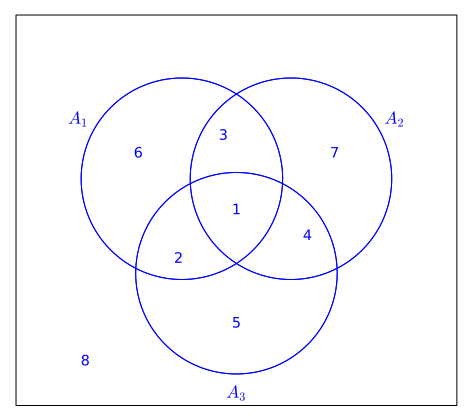
\includegraphics[width=1\linewidth]{images/sageplot-venn-CS_Students.pdf}}%
{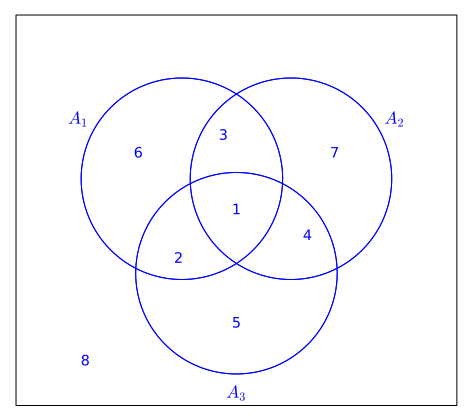
\includegraphics[width=1\linewidth]{images/sageplot-venn-CS_Students.png}}
\caption{Venn Diagram\label{venn_diagram_CS_Students}}
\end{figure}
\par

 We see that the whole universal set is naturally partitioned into subsets that are labeled by the numbers 1 through 8, and the set \(A\)  is  partitioned into subsets labeled 1 through 7. The region labeled 8 represents all students who are not junior CS majors.  Note also that students in the subsets labeled 2, 3, and 4 are double counted, and those in the subset labeled 1 are triple counted. To adjust, we must subtract the numbers in regions 2, 3 and 4.  This can be done by subtracting the numbers in the intersections of each pair of sets.  However, the individuals in region 1 will have been removed three times, just as they had been originally added three times.  Therefore, we must finally add their number back in.
%
\par
\begin{equation*}
\begin{split}
 \lvert A \rvert & =  \lvert A_1 \cup A_2 \cup A_3 \rvert \\ 
 & = \lvert A_1 \rvert + \lvert A_2 \rvert + \lvert A_3 \rvert - \textrm{repeats} \\
 & = \lvert A_1 \rvert + \lvert A_2 \rvert + \lvert A_3 \rvert - \textrm{duplicates} + \textrm{triplicates}  \\
 & = \lvert A_1 \rvert + \lvert A_2 \rvert + \lvert A_3 \rvert - \left(\lvert A_1 \cap A_2 \rvert + \lvert A_1 \cap A_3 \rvert+ \lvert A_2 \cap A_3 \rvert \right) + \lvert A_1 \cap A_2 \cap A_3 \rvert  \\
 & = 75 + 60 + 55 - 25 - 12 - 15 + 10 = 148 
\end{split}
\end{equation*}
%
\end{example}
\par

The ideas used in this latest example gives rise to a basic counting technique:
%
\begin{theorem}[Laws of Inclusion-Exclusion]\label{inclusion-exclusion}
\index{Inclusion-Exclusion, Laws of }Given finite sets \(A_1, A_2, A_3\), then%
\par
\leavevmode%
\begin{enumerate}
\item\hypertarget{ie2}{}\begin{equation*} \lvert A_1 \cup A_2 \rvert =\lvert A_1 \rvert + \lvert A_2 \rvert - \lvert A_1 \cap A_2 \rvert  \end{equation*}%
\item\hypertarget{ie3}{}
\begin{equation*} 
\begin{split}
 \lvert A_1 \cup A_2 \cup A_3 \rvert & =\lvert A_1 \rvert + \lvert A_2 \rvert + \lvert A_3 \rvert\\
&\quad - (\lvert A_1 \cap A_2 \rvert + \lvert A_1 \cap A_3 \rvert+ \lvert A_2 \cap A_3 \rvert)\\
&\quad + \lvert A_1 \cap A_2 \cap A_3 \rvert
\end{split} 
\end{equation*}%
\end{enumerate}
%
\end{theorem}
\par
The inclusion-exclusion laws extend to more than three sets, as will be explored in the exercises.%
\par
In this section we saw that being able to partition a set into disjoint subsets gives rise to a handy counting technique. Given a set, there are many ways to partition depending on what one would wish to accomplish. One natural partitioning of sets is apparent when one draws a Venn diagram. This particular partitioning of a set will be discussed further in Chapters 4 and 13.
%
\typeout{************************************************}
\typeout{Exercises 1.3.1 Exercises for Section 2.3}
\typeout{************************************************}
\subsection[Exercises for Section 2.3]{Exercises for Section 2.3}\label{exercises-2-3}
\hypertarget{exercisegroup-5}{}\typeout{************************************************}
\typeout{Introduction  }
\typeout{************************************************}
A Exercises%
\begin{exercisegroup}
\item[1.]\hypertarget{exercise-32}{} List all partitions of the set \(A =\{a, b, c\}\).%
\par\smallskip
\par\smallskip
\noindent\textbf{Answer.}\hypertarget{answer-17}{}\quad
 \(\{\{a\}, \{b\}, \{c\}\}, \{\{a, b\}, \{c\}\}, \{\{a, c\}, \{b\}\}, \{\{a\}, \{b, c\}\}, \{\{a, b, c\}\}\)%
\item[2.]\hypertarget{exercise-33}{}Which of the following collections of subsets of the plane, \( \mathbb{R}^2\), are partitions?%
\par
\leavevmode%
\begin{enumerate}[label=\alph*]
\item\hypertarget{li-48}{}\( \{ \{(x, y) \mid x + y = c \} \mid c \in \mathbb{R} \}\)%
\item\hypertarget{li-49}{} The set of all circles in \( \mathbb{R}^2 \)%
\item\hypertarget{li-50}{} The set of all circles in \(\mathbb{R}^2\) centered at the origin together with the set \(\{(0,0)\}\)%
\item\hypertarget{li-51}{}\(\{\{(x, y)\} \mid (x, y) \in \mathbb{R}^2  \} \)%
\end{enumerate}
%
\par\smallskip
\item[3.]\hypertarget{exercise-34}{}A student, on an exam paper, defined the term partition the following way: ``Let \(A\)  be a set. A partition of \(A\) is any set of nonempty subsets \(A_1, A_2, A_3, \dots\)  of \(A\) such that each element of A is in one of the subsets.''  Is this definition correct? Why?%
\par\smallskip
\par\smallskip
\noindent\textbf{Answer.}\hypertarget{answer-18}{}\quad
 No. By this definition it is possible that an element of \(A\) might belong to two of the subsets.%
\item[4.]\hypertarget{exercise-35}{} Let \(A_1\) and \(A_2\) be subsets of a set \(U\).   Draw a Venn diagram of this situation and shade in the subsets \(A_1 \cap A_2\), \(A_1^c \cap A_2\),\(A_1 \cap A_2^c\),and \(A_1^c \cap A_2^c\) . Use the resulting diagram and the definition of partition to convince yourself that the subset of these four subsets that are nonempty form a partition of \(U\).%
\par\smallskip
\item[5.]\hypertarget{exercise-36}{} Show that \(\{\{2 n \mid n \in \mathbb{Z}\}, \{2 n + 1 \mid n \in \mathbb{Z}\}\}\) is a partition of \(\mathbb{Z}\). Describe this partition using only words.%
\par\smallskip
\par\smallskip
\noindent\textbf{Answer.}\hypertarget{answer-19}{}\quad
 The first subset is all the even integers and the second is all the odd integers.
These two sets do not intersect and they cover the integers completely.%
\item[6.]\hypertarget{exercise-37}{}
\leavevmode%
\begin{enumerate}[label=\alph*]
\item\hypertarget{li-52}{}A group of 30 students were surveyed and it was found that 18 of them took Calculus and 12 took Physics. If all students took at least one course, how many took both Calculus and Physics? Illustrate using a Venn diagram.%
\item\hypertarget{li-53}{}What is the answer to the question in part (a) if five students did not take either of the two courses? Illustrate using a Venn diagram.%
\end{enumerate}

%
\par\smallskip
\item[7.]\hypertarget{exercise-38}{}A survey of 90 people, 47 of them played tennis and 42 of them swam. If 17 of the them participated in both activities, how many of them participated in neither.%
\par\smallskip
\par\smallskip
\noindent\textbf{Answer.}\hypertarget{answer-20}{}\quad
Since 17 participated in both activities, 30 of the tennis players only played tennis and 25 of the swimmers only swam. Therefore, \(17+30+25=72\) of those who were surveyed participated in an activity and so 18 did not.%
\item[8.]\hypertarget{exercise-39}{}A survey of 300 people found that 60 owned an iPhone 75 owned an Blackberry, and 30 owned an Android phone. Furthermore, 40 owned both an iPhone and Blackberry, 12 owned both an iPhone and Android phone, and 8 owned a Blackberry and an Android phone. Finally, 3 owned all three phones.%
\par
\leavevmode%
\begin{enumerate}[label=\alph*]
\item\hypertarget{li-54}{} How many people surveyed owned none of the three phones?%
\item\hypertarget{li-55}{} How many people owned an Blackberry but not an iPhone?%
\item\hypertarget{li-56}{} How many owned a Blackberry but not an Android?%
\end{enumerate}
%
\par\smallskip
\end{exercisegroup}
\par\smallskip\noindent
\hypertarget{exercisegroup-6}{}\typeout{************************************************}
\typeout{Introduction  }
\typeout{************************************************}
B Exercises%
\begin{exercisegroup}
\item[9.]\hypertarget{exercise-40}{}\leavevmode%
\begin{enumerate}[label=\alph*]
\item\hypertarget{li-57}{} Use the \hyperlink{ie2}{Two Set Inclusion-Exclusion Law}  to derive the  \hyperlink{ie3}{Three Set Inclusion-Exclusion Law}. Note: a knowledge of basic set laws is needed for this exercise.%
\item\hypertarget{li-58}{} State and derive the Inclusion-exclusion law for four sets.%
\end{enumerate}
%
\par\smallskip
\par\smallskip
\noindent\textbf{Solution.}\hypertarget{solution-1}{}\quad
 We assume that \( \lvert A_1 \cup A_2 \rvert = \lvert A_1 \rvert +\lvert  A_2\rvert  -\lvert A_1\cap A_2\rvert   \).
\begin{equation*}
\begin{split}
\lvert A_1 \cup A_2\cup A_3 \rvert  &  =\lvert (A_1\cup A_2) \cup A_3 \rvert   \quad  Why?\\
	& = \lvert A_1\cup A_2\rvert   +\lvert  A_3 \rvert  -\lvert (A_1\cup A_2)\cap A_3\rvert \quad Why? \\
	& =\lvert (A_1\cup A_2\rvert   +\lvert  A_3\rvert  -\lvert (A_1\cap A_3)\cup (A_2\cap A_3)\rvert \quad Why?\\
	& =\lvert  A_1\rvert  +\lvert  A_2\rvert  -\lvert A_1\cap A_2\rvert   +\lvert  A_3\rvert \\
	& \quad -(\lvert A_1\cap A_3\rvert   +\lvert A_2\cap A_3\rvert   -\lvert (A_1\cap A_3)\cap (A_2\cap A_3)\rvert\quad Why?\\
	& =\lvert  A_1\rvert  +\lvert  A_2\rvert  +\lvert  A_3\rvert  -\lvert A_1\cap A_2\rvert -\lvert A_1\cap A_3\rvert\\
	& \quad  -\lvert A_2\cap A_3\rvert +\lvert A_1\cap A_2\cap A_3\rvert \quad Why?  
\end{split}
\end{equation*}
%
\par
 The law for four sets is  
\begin{equation*}
\begin{split}
\lvert A_1\cup A_2\cup A_3\cup A_4\rvert  & =\lvert  A_1\rvert  +\lvert  A_2\rvert  +\lvert  A_3\rvert  +\lvert  A_4\rvert\\
	& \quad  -\lvert A_1\cap A_2\rvert  -\lvert A_1\cap A_3\rvert  -\lvert A_1\cap A_4\rvert \\
	& \quad \quad -\lvert A_2\cap A_3\rvert   -\lvert A_2\cap A_4\rvert -\lvert A_3\cap A_4\rvert   \\
	& \quad +\lvert A_1\cap A_2\cap A_3\rvert +\lvert A_1\cap A_2\cap A_4\rvert   \\
   & \quad \quad +\lvert A_1\cap A_3\cap A_4\rvert +\lvert A_2\cap A_3\cap A_4\rvert \\
   & \quad   -\lvert A_1\cap A_2\cap A_3\cap A_4\rvert  
\end{split}
\end{equation*}
%
\par
Derivation:
\begin{equation*}
\begin{split}
\lvert A_1\cup A_2\cup A_3\cup A_4\rvert & = \lvert (A_1\cup A_2\cup A_3)\cup A_4\rvert  \\
   & = \lvert  (A_1\cup A_2\cup A_3\rvert   +\lvert  A_4\rvert  -\lvert (A_1\cup A_2\cup A_3)\cap A_4\rvert\\
   & = \lvert  (A_1\cup A_2\cup A_3\rvert   +\lvert  A_4\rvert \\
   & \quad -\lvert (A_1\cap A_4)\cup (A_2\cap A_4)\cup (A_3\cap A_4)\rvert  \\
   & = \lvert  A_1\rvert  +\lvert  A_2\rvert  +\lvert  A_3\rvert  -\lvert A_1\cap A_2\rvert  -\lvert A_1\cap A_3\rvert  \\
   & \quad -\lvert A_2\cap A_3\rvert   +\lvert A_1\cap A_2\cap A_3\rvert   +\lvert  A_4\rvert  -\lvert A_1\cap A_4\rvert    \\
   & \quad+\lvert A_2\cap A_4\rvert   +\lvert A_3\cap A_4\rvert  -\lvert (A_1\cap A_4)\cap (A_2\cap A_4)\rvert  \\
   & \quad  -\lvert (A_1\cap A_4)\cap (A_3\cap A_4)\rvert   -\lvert (A_2\cap A_4)\cap (A_3\cap A_4)\rvert \\
   & \quad  +\lvert (A_1\cap A_4)\cap (A_2\cap A_4)\cap (A_3\cap A_4)\rvert  \\
   & =\lvert  A_1\rvert  +\lvert  A_2\rvert  +\lvert  A_3\rvert  +\lvert  A_4\rvert  -\lvert A_1\cap A_2\rvert   -\lvert A_1\cap A_3\rvert   \\
   & \quad  -\lvert A_2\cap A_3\rvert   -\lvert A_1\cap A_4\rvert   -\lvert A_2\cap A_4\rvert  \quad  -\lvert A_3\cap A_4\rvert  \\
   & \quad  +\lvert A_1\cap A_2\cap A_3\rvert  +\lvert A_1\cap A_2\cap A_4\rvert  \\
   & \quad  +\lvert A_1\cap A_3\cap A_4\rvert  +\lvert A_2\cap A_3\cap A_4\rvert \\
   & \quad     -\lvert A_1\cap A_2 \cap A_3\cap A_4\rvert 
\end{split}   
\end{equation*}
%
\item[10.]\hypertarget{exercise-41}{} To complete your spring schedule, you must add Calculus and Physics. At 9:30, there are three Calculus sections and two Physics sections; while at 11:30, there are two Calculus sections and three Physics sections.  How many ways can you complete your schedule if your only open periods are 9:30 and 11:30?%
\par\smallskip
\end{exercisegroup}
\par\smallskip\noindent
\hypertarget{exercisegroup-7}{}\typeout{************************************************}
\typeout{Introduction  }
\typeout{************************************************}
C Exercise%
\begin{exercisegroup}
\item[11.]\hypertarget{exercise-42}{}The definition of \(\mathbb{Q}  = \{a/b \mid a, b \in \mathbb{Z}, b \neq 0\}\) given in Chapter 1 is  awkward. If we use the definition to list elements in \(\mathbb{Q}\), we will have duplications such as \(\frac{1}{2}\), \(\frac{-2}{-4}\) and \(\frac{300}{600}\)   Try to write a more precise definition of the rational numbers so that there is no duplication of elements.%
\par\smallskip
\par\smallskip
\noindent\textbf{Answer.}\hypertarget{answer-21}{}\quad
Partition the set of fractions into blocks, where each block contains fractions that are numerically equivalent. Describe how you would determine whether two fractions belong to the same block. Redefine the rational numbers to be this partition. Each rational number is a set of fractions.%
\end{exercisegroup}
\par\smallskip\noindent
\typeout{************************************************}
\typeout{Section 1.4 Combinations and the Binomial Theorem}
\typeout{************************************************}
\section[Combinations and the Binomial Theorem]{Combinations and the Binomial Theorem}\label{combinations-and-the-binomial-theorem}
\typeout{************************************************}
\typeout{Subsection 1.4.1 Combinations}
\typeout{************************************************}
\subsection[Combinations]{Combinations}\label{combinations}
\index{Combinations} In Section 2.1 we investigated the most basic concept in combinatorics, namely, the rule of products. Even though in this section we investigate other counting formulas, it is of paramount importance to keep this fundamental process in mind. In Section 2.2 we saw that a subclass of rule-of-products problems appears so frequently that we gave them a special designation, namely, permutations, and we derived a formula as a computational aid to assist us. In this section we will investigate another counting formula that are used to count combinations, which are subsets of a certain size..%
\par
In many rule-of-products applications the permutation or order is important, as in the situation of the order of putting on one's socks and shoes; in some cases it is not important, as in placing coins in a vending machine or in the listing of the elements of a set. Order is important in permutations. Order is not important in combinations.%
\begin{example}[Counting Permutations]\label{counting-permuations-multiple-ways}
How many different ways are there to permute three letters from the set \(A = \{a, b, c, d\}\)?  From the \hyperref[permutations-counting-formula]{Permutation Counting Formula} there are \(P(4,3)=\frac{4!}{(4-3)!} = 24\) different orderings of three letters from \(A\) %
\end{example}
\begin{example}[Counting with No Order]\label{four-choose-three}
How many ways can we select a set of three letters from  \(A = \{a, b, c, d\}\)?  Note here that we are not concerned with the order of the three letters. By trial and error, abc, abd, acd, and bcd are the only listings possible. To repeat, we were looking for all three-element subsets of the set A. Order is not important in sets. The notation for choosing 3 elements from 4 is most commonly \(\binom{4}{3}\) or occasionally \(C(4,3)\), either of which is read ``4 choose 3'' or the number of combinations for four objects taken three at a time.%
\end{example}
\begin{definition}[Binomial Coefficient]\label{binomial-coefficient}
\index{Binomial Coefficient}\label{notation-2}
Let \(n\) and \(k\) be nonnegative integers.  The binomial coefficient \(\binom{n}{k}\) represents the number of combinations of \(n\) objects taken \(k\) at a time, and is read ``\(n\) choose \(k\).''%
\end{definition}
\par
We would now like to investigate the relationship between permutation and combination problems in order to derive a formula for \(\binom{n}{k}\)%
\par
Let us reconsider the \hyperref[four-choose-three]{Counting with No Order}. There are \(3 ! = 6\) different orderings for each of the three-element subsets. The table below lists each subset of \(A\)  and all permutations of each subset on the same line.
\begin{equation*}
 \begin{array}{cc}
 \textrm{subset} & \textrm{permutations} \\
 abc & abc,acb,bca,bac,cab,cba \\
 abd & abd,adb,bda,bad,dab,dba \\
 acd & acd,adc,cda,cad,dac,dca \\
 bcd & bcd,bdc,cdb,cbd,dbc,dcb \\
\end{array}
 \end{equation*}%
\par
 Hence, \(\binom{4}{3} = \frac{P(4,3)}{3!} = \frac{4!}{(4-3)! \cdot 3!} = 4\)%
\par
 We generalize this result in the following theorem:%
\begin{theorem}[Binomial Coefficient Formula]\label{binomial-coefficient-formula}
\index{Binomial Coefficient Formula}If \(n\) and \(k\) are nonnegative integers with \(0 \leq k \leq n\), then the number \(k\)-element subsets of an \(n\) element set is equal to \begin{equation*}\binom{n}{k} = \frac{n!}{(n-k)! \cdot k!} \end{equation*}%
\end{theorem}
\begin{proof}\hypertarget{proof-3}{}
Proof 1: There are \(k!\) ways of ordering the elements of any \(k\) element set.Therefore,
\begin{equation*}\binom{n}{k} = \frac{P(n,k)}{k!} = \frac{n!}{(n-k)! k!}.\end{equation*}%
\par
Proof 2: To ``construct'' a permutation of \(k\)  objects from a set of \(n\) elements, we can first choose one of the subsets of objects and second, choose one of the \(k!\)  permutations of those objects. By the rule of products,\begin{equation*}P(n,k) = \binom{n}{k} \cdot k!\end{equation*} and solving for \(\binom{n}{k}\) we get the desired formula.%
\end{proof}
\begin{example}[Flipping Coins]\label{flipping-coins}
  Assume an evenly balanced coin is tossed five times. In how many ways can three heads be obtained? This is a combination problem, because the order in which the heads appear does not matter. The number of ways to get three heads is \(\binom{5}{3}= \frac{5 \cdot 4}{2 \cdot 1} = 10\).
%
\end{example}
\begin{example}[Listing Five Flips, taking order into account]\label{five-flips}
Determine the total number of ways a fair coin can land if tossed five consecutive times. The five tosses can produce any one of the following mutually exclusive, disjoint events: 5 heads, 4 heads, 3 heads, 2 heads, 1 head, or 0 heads. Hence by the law of addition we have:
\begin{equation*}\binom{5}{5}+\binom{5}{4}+\binom{5}{3}+\binom{5}{2}+\binom{5}{1}+\binom{5}{0}= 1 + 5 +10+10+5+1 = 32\end{equation*} ways to observe the five flips%
\par
 Of course, we could also have applied the extended rule of products, and since there are two possible outcomes for each of the five tosses, we have \(2^5 = 32\) ways.%
\end{example}
\par
You might think that counting something two ways is a waste of time but solving a problem two different ways often is instructive and leads to valuable insights. In this case, it suggests a general formula for the sum 
\(\sum_{k=0}^n \binom{n}{k}\). In the case of \(n = 5\), we get \(2^5\) so it is reasonable to expect that the general sum is \(2^n\), and it is.%
\begin{example}[A Committee of Five]\label{committee-of-five}
A committee usually starts as an unstructured set of people selected from a larger membership. Therefore, a committee can be thought of as a combination. If a club of 25 members has a five-member social committee, there are \(\binom{25}{5}=\frac{25 24 23 22 21}{5!} = 53130\) different possible social committees. If any structure or restriction is placed on the way the social committee is to be selected, the number of possible committees will probably change. For example, if the club has a rule that the treasurer must be on the social committee, then the number of possibilities is reduced to \(\binom{24}{4}=\frac{24 23 22 21}{4!} = 10626\). %
\par
 If we further require that a chairperson other than the treasurer be selected for the social committee, we have  \(\binom{24}{4} \cdot 4 = 42504\) different possible social committees. The choice of the four non-treasurers accounts for the factor \(\binom{24}{4}\) while the need to choose a chairperson accounts for the 4.%
\end{example}
\begin{example}[Binomial Coefficients - Extreme Cases]\label{extreme-binomial-cases}
By simply applying the definition of a \hyperref[binomial-coefficient]{Binomial Coefficient} as a number of subsets we see that there is \(\binom{n}{0} = 1\) way of choosing a combination of zero elements from a set of \(n\). In addition, we see that   there is \(\binom{n}{n} = 1\) way of choosing a combination of \(n\) elements from a set of \(n\). %
\par
We could compute these values using the formula we have developed, but no arithmetic is really needed here.  Other properties of binomial coefficients that can be derived using the subset definition will be seen in the exercises%
\end{example}
\typeout{************************************************}
\typeout{Subsection 1.4.2 The Binomial Theorem}
\typeout{************************************************}
\subsection[The Binomial Theorem]{The Binomial Theorem}\label{the-binomial-theorem}

 The binomial theorem gives us a formula for expanding \(( x + y )^{n}\), where \(n\)  is a nonnegative integer. The coefficients of this expansion are precisely the binomial coefficients that we have used to count combinations. Using high school algebra we can  expand the expression for integers from 0 to 5:%
\par
\begin{equation*} \begin{array}{cc}
 n & (x + y)^n \\
 0 & 1 \\
 1 & x+y \\
 2 & x^2+2 x y+y^2 \\
 3 & x^3+3 x^2 y+3 x y^2+y^3 \\
 4 & x^4+4 x^3 y+6 x^2 y^2+4 x y^3+y^4
   \\
 5 & x^5+5 x^4 y+10 x^3 y^2+10 x^2
   y^3+5 x y^4+y^5 \\
\end{array}
 \end{equation*}
 %
\par
In the expansion of \((x + y)^{5} \)  we note that the coefficient of the third term is \(\binom{5}{3} = 10\), and that of the sixth term is  \(\binom{5}{5}=1\). We can rewrite the expansion as 
\begin{equation*}\binom{5}{0} x^5+\binom{5}{1} x^4 y+\binom{5}{2} x^3 y^2+\binom{5}{3} x^2 y^3+\binom{5}{4} x y^4+ \binom{5}{5} y^5
\end{equation*}%
\par

 In summary, in the expansion of \(( x + y )^{n}\) we note:%
\par
\leavevmode%
\begin{enumerate}
\item\hypertarget{li-59}{}The first term is \(x^n\) and the last term is \(y^n\). %
\item\hypertarget{li-60}{} With each successive term, exponents of \(x\) decrease by 1 as those of \(y\) increase by 1. For any term the sum of the exponents is \(n\).%
\item\hypertarget{li-61}{}  The coefficient of \(x^{n-k} y^k\) is \(\binom{n}{k}\).%
\item\hypertarget{li-62}{} The triangular array of binomial coefficients is called Pascal's triangle after the seventeenth-century French mathematician Blaise Pascal. Note that each number in the triangle other than the 1's at the ends of each row is the sum of the two numbers to the right and left of it in the row above.%
\end{enumerate}
%
\begin{theorem}[The Binomial Theorem]\label{binomial-theorem}
\index{The Binomial Theorem} If \(n \geq  0\), and \(x\) and \(y\) are numbers, then
\begin{equation*}(x+y)^{n} = \sum_{k=0}^n \binom{n}{k} x^{n-k} y^k\end{equation*}%
\end{theorem}
\begin{proof}\hypertarget{proof-4}{}
This theorem will proven using a logical procedure called mathematical induction, which will be introduced in Chapter 3. %
\end{proof}
\begin{example}[Identifying a term in an expansion]\label{term-in-an-expansion}
Find the third term in the expansion of \(( x-y )^{4}\). The third term,  when \(k=2\), is \(\binom{4}{2} x^{4-2} y^2 = 6 x^2 y^2\).%
\end{example}
\begin{example}[A Binomial Expansion]\label{a-full-expansion}

Expand \((3 x - 2 )^{3}\).  If we replace \(x\)  and \(y\)  in the Binomial Theorem with \(3x\) and \(-2\), respectively, we get
\begin{equation*}\begin{split} 
\sum_{k=0}^3 \binom{3}{k} (3x)^{n-k} (-2)^k & = \binom{3}{0} (3x)^{3} (-2)^0 + \binom{3}{1} (3x)^{2} (-2)^1 + \binom{3}{2} (3x)^{1} (-2)^2 + \binom{3}{3} (3x)^{0} (-2)^3 \\
& = 27 x^3 - 54 x^2 + 36 x - 8 
\end{split}
\end{equation*}%
\end{example}
\typeout{************************************************}
\typeout{Subsection 1.4.3 \emph{Mathematica}  Note}
\typeout{************************************************}
\subsection[\emph{Mathematica}  Note]{\emph{Mathematica}  Note}\label{mathematica-binomial}
\index{Mathematica  Note!Bridge Hands}\emph{Mathematica}  has a built-in function for binomial coefficients, \(\texttt{Binomial}\). Unlike the examples we've concentrated on that can be done without technology, you can compute extremely large values. For 
example, a bridge hand is a 13 element subset of a standard 52 card deck. The order in which the cards come to the player doesn't matter. From the point of view of a single player, the number of possible bridge hands is \(\texttt{Binomial[52,13]}\), which is easily computed with \(Mathematica\) with an output of 635013559600%
\par
In bridge, the location of a hand in relation to the dealer has some bearing on the game. An even truer indication of the number of possible hands takes into account \(each\)  player's possible hand. It is customary 
to refer to bridge positions as West, North, East and South. We can apply the rule of product to get the total number of bridge hands with the following logic. West can get any of the \(\binom{52}{13}\) hands identified above. Then North get 13 of the remaining 39 cards and so has  \(\binom{39}{13}\) possible hands. East then gets 13 of the 26 remaining cards, which has \(\binom{26}{13}\)  possibilities. South gets the remaining cards. Therefore the number of bridge hands is computed by evaluating the expression \begin{equation*}\texttt{Binomial[52,13] Binomial[52,13] Binomial[52,13]}\end{equation*} which is equal to 53644737765488792839237440000%
\typeout{************************************************}
\typeout{Subsection 1.4.4 Sage Note}
\typeout{************************************************}
\subsection[Sage Note]{Sage Note}\label{sage-bridge-hands}
\index{Sage Note!bridge hands}
 Sage will do the same calculations for bridge hands just as easily. A correct input is provided in the sage cell below. 
%
\begin{lstlisting}[style=sageinput]
binomial(52,13)*binomial(39,13)*binomial(26,13)
\end{lstlisting}
\begin{lstlisting}[style=sageoutput]
53644737765488792839237440000
\end{lstlisting}
\typeout{************************************************}
\typeout{Exercises 1.4.5 Exercises}
\typeout{************************************************}
\subsection[Exercises]{Exercises}\label{exercises-2-4}
\hypertarget{exercisegroup-8}{}\typeout{************************************************}
\typeout{Introduction  }
\typeout{************************************************}
A Exercises%
\begin{exercisegroup}
\item[1.]\hypertarget{exercise-43}{} The judiciary committee at a college is made up of three faculty members and four students. If ten faculty members and 25 students have been nominated for the committee, how many judiciary committees could be formed at this point	?%
\par\smallskip
\par\smallskip
\noindent\textbf{Answer.}\hypertarget{answer-22}{}\quad
 \(C(10,3)\cdot C(25,4)=1,518,000\)%
\item[2.]\hypertarget{exercise-44}{} Suppose that a single character is stored in a computer using eight bits.%
\par
a. How many bit patterns have exactly three 1 's?%
\par
b. How many bit patterns have at least two 1 's?%
\par\smallskip
\par\smallskip
\noindent\textbf{Hint.}\hypertarget{hint-1}{}\quad
Think of the set of positions that contain a 1 to turn this is into a question about sets.%
\par\smallskip
\noindent\textbf{Solution.}\hypertarget{solution-2}{}\quad
(a) \(\binom{8}{3}\) (b) \(2^8-(\binom{8}{0}+\binom{8}{1})\)%
\item[3.]\hypertarget{exercise-45}{} How many subsets of \(\{1, 2, 3, \dots , 10\}\) contain at least seven elements?%
\par\smallskip
\par\smallskip
\noindent\textbf{Answer.}\hypertarget{answer-23}{}\quad
 \(C(10,7)+C(10,8)+C(10,9)+C(10,10)\) %
\item[4.]\hypertarget{exercise-46}{} The congressional committees on mathematics and computer science are made up of five congressmen each, and a congressional rule is that the two committees must be disjoint. If there are 385 members of congress, how many ways could the committees be selected?%
\par\smallskip
\item[5.]\hypertarget{exercise-47}{}Expand \( ( 2x - 3y )^4\)%
\par\smallskip
\par\smallskip
\noindent\textbf{Answer.}\hypertarget{answer-24}{}\quad
 \(16x^4-96x ^3y+216x^2y^2-216x y^3+81y^4\)%
\item[6.]\hypertarget{exercise-48}{}Find the fourth term of the expansion of \((x -2y)^6\).%
\par\smallskip
\item[7.]\hypertarget{exercise-49}{}(a) A poker game is played with 52 cards. How many ``hands'' of five cards are possible?%
\par
(b) If there are four people playing, how many five-card ``hands'' are possible on the first deal?%
\par\smallskip
\par\smallskip
\noindent\textbf{Answer.}\hypertarget{answer-25}{}\quad
\leavevmode%
\begin{enumerate}[label=\alph*]
\item\hypertarget{li-63}{} \(C(52,5)=2,598,960\)%
\item\hypertarget{li-64}{}  \(C(52,5)\cdot C(47,5)\cdot C(42,5)\cdot C(37,5)\)%
\end{enumerate}
%
\item[8.]\hypertarget{exercise-50}{} A flush in a five-card poker hand is five cards of the same suit. How many spade flushes are possible in a 52-card deck? How many flushes are possible in any suit?%
\par\smallskip
\item[9.]\hypertarget{exercise-51}{} How many five-card poker hands using 52 cards contain exactly two aces?%
\par\smallskip
\par\smallskip
\noindent\textbf{Answer.}\hypertarget{answer-26}{}\quad
\(C(4,2)C(48,3)\)%
\item[10.]\hypertarget{exercise-52}{}  In poker, a full house is three-of-a-kind and a pair in one hand; for example, three fives and two queens. How many full houses are possible from a 52-card deck?  You can use the sage cell in the \hyperref[sage-bridge-hands]{Sage Note} to do this calculation, but also write your answer in terms of binomial coefficients. %
\par\smallskip
\item[11.]\hypertarget{exercise-53}{} A class of twelve computer science students are to be divided into three groups of 3, 4, and 5 students to work on a project. How many ways can this be done if every student is to be in exactly one group?%
\par\smallskip
\par\smallskip
\noindent\textbf{Answer.}\hypertarget{answer-27}{}\quad
\(C(12,3)\cdot C(9,4)\cdot C(5,5)\)%
\end{exercisegroup}
\par\smallskip\noindent
\hypertarget{exercisegroup-9}{}\typeout{************************************************}
\typeout{Introduction  }
\typeout{************************************************}
B Exercises%
\begin{exercisegroup}
\item[12.]\hypertarget{exercise-54}{} Explain in words why the following equalities are true based on number of subsets,  and then verify the equalities using the formula for binomial coefficients.%
\par
\leavevmode%
\begin{enumerate}[label=\alph*]
\item\hypertarget{li-65}{}\(\binom{n}{1} = n\) %
\item\hypertarget{li-66}{}\(\binom{n}{k} = \binom{n}{n-k}\), \( 0 \leq k \leq n\)%
\end{enumerate}
%
\par\smallskip
\item[13.]\hypertarget{exercise-55}{}  There are ten points, \(P_1, P_2, \dots , P_{10}\) on a plane, no three on the same line.%
\par
\leavevmode%
\begin{enumerate}[label=\alph*]
\item\hypertarget{li-67}{}How many lines are determined by the points?%
\item\hypertarget{li-68}{} How many triangles are determined by the points?%
\end{enumerate}
%
\par\smallskip
\par\smallskip
\noindent\textbf{Answer.}\hypertarget{answer-28}{}\quad
\leavevmode%
\begin{enumerate}[label=\alph*]
\item\hypertarget{li-69}{} \(C(10,2)=45\)%
\item\hypertarget{li-70}{} \(C(10,3)=120\)%
\end{enumerate}
%
\item[14.]\hypertarget{exercise-56}{} How many ways can \(n\)  persons be grouped into pairs when \(n\)  is even? Assume the order of the pairs matters, but not the order within the pairs. For example, if \(n=4\), the six different groupings would be
\begin{equation*}\begin{array}{cc}
 \{1,2\} & \{3,4\} \\
 \{1,3\} & \{2,4\} \\
 \{1,4\} & \{2,3\} \\
 \{2,3\} & \{1,4\} \\
 \{2,4\} & \{1,3\} \\
 \{3,4\} & \{1,2\} \\
\end{array}
\end{equation*} %
\par\smallskip
\item[15.]\hypertarget{exercise-57}{} Use the binomial theorem to prove that if \(A\) is a finite set, then 
\(\mathscr{P}(A) = 2^{\lvert A \rvert}\)%
\par\smallskip
\par\smallskip
\noindent\textbf{Answer.}\hypertarget{answer-29}{}\quad
 Assume \(\lvert A \rvert =n.\) If we let \(x=y=1\) in the Binomial Theorem, we obtain \(2^n=C(n;0)+C(n;1)+\cdots +C(n;n)\), with the right side of the equality counting all subsets of \(A\) containing \(0, 1, 2, \dots , n\) elements.  Hence \(\left| P(A)\right| =2^{\left| A\right| }\) %
\item[16.]\hypertarget{exercise-58}{}\leavevmode%
\begin{enumerate}[label=\alph*]
\item\hypertarget{li-71}{}A state's lottery involves choosing six different numbers out of a possible 36. How many ways can a person choose six numbers?%
\item\hypertarget{li-72}{}What is the probability of a person winning with one bet?%
\end{enumerate}
%
\par\smallskip
\item[17.]\hypertarget{exercise-59}{}Use the binomial theorem to calculate \(9998^3\).%
\par\smallskip
\par\smallskip
\noindent\textbf{Hint.}\hypertarget{hint-2}{}\quad
\(9998 = 10000-2\)%
\par\smallskip
\noindent\textbf{Answer.}\hypertarget{answer-30}{}\quad
 \(1000^3 - 3\cdot 2 \cdot 1000^2 +3 \cdot 2^2 \cdot 1000 -2^3 = 999,400,119,992.\)%
\item[18.]\hypertarget{exercise-60}{} In the card game Blackjack, there are one or more players and a dealer.  Initially, each player is dealt two cards and the dealer is dealt one card down and one facing up.  As in bridge, the order of the hands, but not the order of the cards in the hands, matters.  Starting with a single 52 card deck, and three players, how many ways can the first two cards be dealt out?  You can use the sage cell in the \hyperref[sage-bridge-hands]{Sage Note} to do this calculation. %
\par\smallskip
\end{exercisegroup}
\par\smallskip\noindent
%
\backmatter
%
%
%% A lineskip in table of contents as transition to appendices, backmatter
\addtocontents{toc}{\vspace{\normalbaselineskip}}
%
\typeout{************************************************}
\typeout{References  References}
\typeout{************************************************}
\chapter[References]{References}\label{references-1}
%% If this is a top-level references
%%   you can replace with "thebibliography" environment
\begin{referencelist}
\bibitem[1]{biblio-sopowit-1983}\hypertarget{biblio-sopowit-1983}{}Sopowit, K. J., E. M. Reingold, and D. A. Plaisted \textit{The Traveling Salesman Problem and Minimum Matching in the Unit Square}.SIAM J. Computing, 1983,\textbf{12}, 144\textendash{}56.
\end{referencelist}
%
%% The index is here, setup is all in preamble
\printindex
%
\end{document}